
\begin{frame}
  \frametitle{What is PDE-constrained optimisation?}

  \emph{Optimisation problems where at least one constrained is a partial differential equation}

  \onslide<2>{
  \begin{block}{Applications}
      \begin{itemize}
          \item Data assimilation.\\ \emph{Example}: Weather modelling.
          \item Shape and topology optimisation.\\ \emph{Example}: Optimal shape of an aerfoil.
          \item Parameter estimation.
          \item Optimal control. 
          \item ...
      \end{itemize}
  \end{block}
  }

\end{frame}

\begin{frame}
    \frametitle{\emph{Hello World} of PDE-constrained optimisation!}

  We will solve the optimal control of the Poisson equation:

  \begin{equation*}
    \begin{split}
        \min_{u, m} & \frac{1}{2} \int_\Omega \| u - u_d\|^2\dx + \frac{\alpha}{2} \int_\Omega \| m \|^2\dx \\
        \textrm{subject to} & \\
      - \Delta u &= m \,\,\, \quad \mbox{in } \Omega
      \\
    u &= u_0 \quad \mbox{on } \partial \Omega
    \end{split}
  \end{equation*}

  \onslide<2->{
  \begin{itemize}
  \item
      This problem can be physically interpreted as:
      Find the heating/cooling term $m$ for which $u$ best approximates the desired heat distribution $u_d$.
  \item
      The second term in the objective functional, known as Thikhonov regularisation, ensures existence and uniqueness for $\alpha >0$.
  \end{itemize}
  }
\end{frame}



\begin{frame}
\frametitle{The canconical abstract form}
  \begin{equation*}
    \begin{split}
        \min_{u, m} J(u, m) \\
        \textrm{subject to: } & \\
        F(u, m) = 0, \\
  %      l_b \le m \le u_b, \\
  %      g(m) \ge 0, \\
  %      h(m) = 0, \\
    \end{split}
  \end{equation*}

  with
  \begin{itemize}
  \item the objective functional $J$.
  \item the parameter $m$.
  \item the PDE operator $F$ with solution $u$, parametrised by $m$.
  %\item bound constraints $\l_b \le m \le u_b$.
  %\item inequality constraints $g$.
  %\item equality constraints $h$.
  \end{itemize}
\end{frame}

\begin{frame}
\frametitle{The reduced problem}
  \begin{equation*}
    \begin{split}
        \min_{m} \tilde J(m) &= J(u(m), m) \\
  %      \textrm{subject to:} & \\
   %     g(m) \ge 0, \\
   %     h(m) = 0, \\
    \end{split}
  \end{equation*}

  with
  \begin{itemize}
  \item the reduced functional $\tilde J$.
  \item the parameter $m$.
  %\item bound constraints $\l_b \le m \le u_b$.
  %\item inequality constraints $g$.
  %\item equality constraints $h$.
  \end{itemize}

  \onslide<2->{
  \begin{block}{How do we solve this problem?}
      \begin{itemize}
          \item Gradient descent.
          \item Newton method.
          \item Quasi-Newton methods.
      \end{itemize}
  \end{block}
  }
\end{frame}

\begin{frame}
\frametitle{Gradient descent}
\begin{block}{Algorithm}
\begin{enumerate}
    \item Choose initial parameter value $m^0$ and $\gamma >0$.
    \item For $i = 0, 1, \dots$:
    \begin{itemize}
        \item $m^{i+1} = m^i -\gamma \nabla J(m^i)$
    \end{itemize}
\end{enumerate}
\end{block}

\begin{figure}
\begin{center}
    \hfill 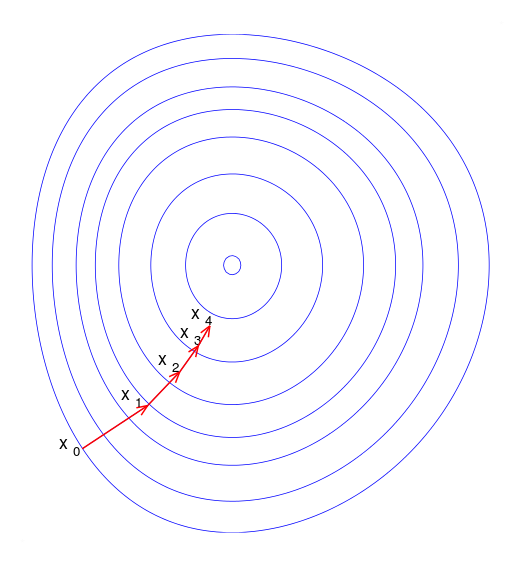
\includegraphics[width=0.4\textwidth]{png/gradient_descent} 
\end{center}
\end{figure}
\vspace{-2cm}
\begin{block}{Features}
\begin{description}
    \item[+] Easy to implement.
    \item[--] Slow convergence.
\end{description}
\end{block}
\end{frame}

\begin{frame}
\frametitle{Newton method}

Optimisation problem:
$\min_{m} \tilde J(m)$.

\onslide<2->{
Optimality condition:
\begin{equation}
 \nabla \tilde J(m) = 0.
 \label{eqn:optcon}
\end{equation}
}

\onslide<3->{
Newton method applied to \eqref{eqn:optcon}:
\begin{enumerate}
    \item Choose initial parameter value $m^0$.
    \item For $i = 0, 1, \dots$:
    \begin{itemize}
        \item $H(J) \delta m = - \nabla J(m^i)$, where $H$ denotes the Hessian.
        \item $m^{i+1} = m^i +\delta m$
    \end{itemize}
\end{enumerate}
}


\onslide<4->{
\begin{block}{Features}
\begin{description}
    \item[+] Fast (locally quadratic) convergence.
    \item[--] Requires iteratively solving a linear system with the Hessian, which might require many Hessian action computations.
    \item[--] Hessian might not be positive definite, resulting in an update $\delta m$ which is not a descent direction.
\end{description}
\end{block}
}
\end{frame}

\begin{frame}
\frametitle{Quasi-Newton methods}

Like Newton method, but use approximate, low-rank Hessian approximation using gradient information only. A common approximation method is \emph{BFGS}.

\onslide<2->{
\begin{block}{Features}
\begin{description}
    \item[+] Robust: Hessian approximation is always positive definite.
    \item[+] Cheap: No Hessian computation required, only gradient computations.
    \item[--] Only superlinear convergence rate.
\end{description}
\end{block}
}

\end{frame}

\begin{frame}[fragile]
\frametitle{Solving the optimal Poisson problem}

\begin{python}
from fenics import *
from dolfin_adjoint import *

# Solve Poisson problem
# ...

J = Functional(inner(s, s)*dx)
m = SteadyParameter(f)

rf = ReducedFunctional(J, m)
m_opt = minimize(rf, method="L-BFGS-B", tol=1e-2)
\end{python}

\onslide<2->{
\begin{block}{Tipps}
\begin{itemize}
    \item You can call \textbf{print\_optimization\_methods()} to list all available methods.
    \item Use \textbf{maximize} if you want to solve a maximisation problem.
\end{itemize}
\end{block}
}

\end{frame}

\begin{frame}[fragile]
\frametitle{Bound constraints}
    Sometimes it is usefull to specify lower and upper bounds for parameters:
    \begin{equation}
        l_b \le m \le u_b.
    \end{equation}

Example:
\begin{python}
lb = interpolate(0, V)
ub = interpolate(Expression("x[0]", degree=1), V)
m_opt = minimize(rf, method="L-BFGS-B", bounds=[lb, ub])
\end{python}
\emph{Note:} Not all optimisation algorithms support bound constraints.
\end{frame}


\begin{frame}[fragile]
\frametitle{Inequality constraints}
Sometimes it is usefull to specify (in-)equality constraints on the parameters:
    \begin{equation}
        g(m) \le 0.
    \end{equation}

You can do that by overloading the \textbf{InequalityConstraint} class. 

For more information visit the \emph{Example} section on \url{dolfin-adjoint.org}.

\end{frame}

\begin{frame}
  \frametitle{\emph{The FEniCS challenge!}}

  \begin{enumerate}
      \item Solve the "Hello world" PDE-constrained optimisation problem on the unit square with 
          $u_d(x, y) = \sin(\pi x)\sin(\pi y)$, homogenous boundary conditions and $\alpha=10^{-6}$.
      \item Compute the difference between optimised heat profile and $u_d$ before and after the optimisation.
      \item Use the optimisation algorithms SLSQP, Newton-CG and L-BFGS-B and compare them.
      \item What happens if you increase $\alpha$?
  \end{enumerate}

\end{frame}

